
%% $Id$

\documentclass[12pt,a4paper,fleqn]{report}
\usepackage{latexsym,graphicx}
\usepackage{listings}
\usepackage[refpage]{nomencl}
\usepackage{../../iman,../../extra,../../isar,../../proof}
\usepackage{Thy/document/isabelle,Thy/document/isabellesym}
\usepackage{style}
\usepackage{Thy/document/pdfsetup}

\newcommand{\cmd}[1]{\isacommand{#1}}

\newcommand{\isasymINFIX}{\cmd{infix}}
\newcommand{\isasymLOCALE}{\cmd{locale}}
\newcommand{\isasymINCLUDES}{\cmd{includes}}
\newcommand{\isasymDATATYPE}{\cmd{datatype}}
\newcommand{\isasymAXCLASS}{\cmd{axclass}}
\newcommand{\isasymFIXES}{\cmd{fixes}}
\newcommand{\isasymASSUMES}{\cmd{assumes}}
\newcommand{\isasymDEFINES}{\cmd{defines}}
\newcommand{\isasymNOTES}{\cmd{notes}}
\newcommand{\isasymSHOWS}{\cmd{shows}}
\newcommand{\isasymCLASS}{\cmd{class}}
\newcommand{\isasymINSTANCE}{\cmd{instance}}
\newcommand{\isasymLEMMA}{\cmd{lemma}}
\newcommand{\isasymPROOF}{\cmd{proof}}
\newcommand{\isasymQED}{\cmd{qed}}
\newcommand{\isasymFIX}{\cmd{fix}}
\newcommand{\isasymASSUME}{\cmd{assume}}
\newcommand{\isasymSHOW}{\cmd{show}}
\newcommand{\isasymNOTE}{\cmd{note}}
\newcommand{\isasymIN}{\cmd{in}}
\newcommand{\isasymCODEGEN}{\cmd{code\_gen}}
\newcommand{\isasymPRINTCODETHMS}{\cmd{print\_codethms}}
\newcommand{\isasymFUN}{\cmd{fun}}
\newcommand{\isasymFUNCTION}{\cmd{function}}
\newcommand{\isasymPRIMREC}{\cmd{primrec}}
\newcommand{\isasymRECDEF}{\cmd{recdef}}

\newcommand{\qt}[1]{``#1''}
\newcommand{\qtt}[1]{"{}{#1}"{}}
\newcommand{\qn}[1]{\emph{#1}}
\newcommand{\strong}[1]{{\bfseries #1}}
\newcommand{\fixme}[1][!]{\strong{FIXME: #1}}

\lstset{basicstyle=\scriptsize\ttfamily, keywordstyle=\itshape, commentstyle=\itshape\sffamily, frame=shadowbox}
\newcommand{\lstsml}[1]{\lstset{language=ML}\lstinputlisting{#1}}
\newcommand{\lsthaskell}[1]{\lstset{language=Haskell}\lstinputlisting{#1}}

\hyphenation{Isabelle}
\hyphenation{Isar}

\isadroptag{theory}
\title{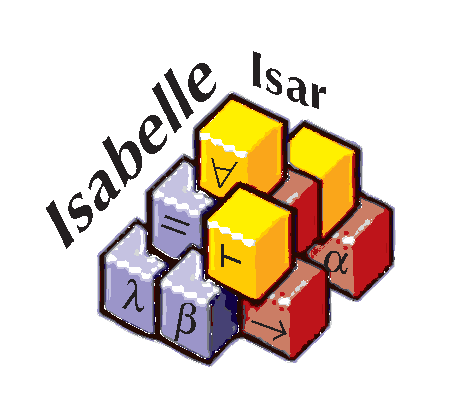
\includegraphics[scale=0.5]{isabelle_isar}
  \\[4ex] Defining Recursive Functions in Isabelle/HOL}
\author{\emph{Alexander Krauss}}


\isabellestyle{tt}

\begin{document}

\maketitle

\begin{abstract}
  This tutorial describes the use of the new \emph{function} package,
  starting with very simple examples and the proceeding to the more
  intricate ones. No familiarity with other definition facilities is
  assumed.
\end{abstract}

\thispagestyle{empty}\clearpage

\pagenumbering{roman}
\clearfirst

%
\begin{isabellebody}%
\def\isabellecontext{Functions}%
%
\isadelimtheory
\isanewline
\isanewline
%
\endisadelimtheory
%
\isatagtheory
\isacommand{theory}\isamarkupfalse%
\ Functions\isanewline
\isakeyword{imports}\ Main\isanewline
\isakeyword{begin}%
\endisatagtheory
{\isafoldtheory}%
%
\isadelimtheory
%
\endisadelimtheory
%
\isamarkupchapter{Defining Recursive Functions in Isabelle/HOL%
}
\isamarkuptrue%
%
\isamarkupsection{Function Definition for Dummies%
}
\isamarkuptrue%
%
\begin{isamarkuptext}%
In most cases, defining a recursive function is just as simple as other definitions:%
\end{isamarkuptext}%
\isamarkuptrue%
\isacommand{fun}\isamarkupfalse%
\ fib\ {\isacharcolon}{\isacharcolon}\ {\isachardoublequoteopen}nat\ {\isasymRightarrow}\ nat{\isachardoublequoteclose}\isanewline
\isakeyword{where}\isanewline
\ \ {\isachardoublequoteopen}fib\ {\isadigit{0}}\ {\isacharequal}\ {\isadigit{1}}{\isachardoublequoteclose}\isanewline
{\isacharbar}\ {\isachardoublequoteopen}fib\ {\isacharparenleft}Suc\ {\isadigit{0}}{\isacharparenright}\ {\isacharequal}\ {\isadigit{1}}{\isachardoublequoteclose}\isanewline
{\isacharbar}\ {\isachardoublequoteopen}fib\ {\isacharparenleft}Suc\ {\isacharparenleft}Suc\ n{\isacharparenright}{\isacharparenright}\ {\isacharequal}\ fib\ n\ {\isacharplus}\ fib\ {\isacharparenleft}Suc\ n{\isacharparenright}{\isachardoublequoteclose}%
\begin{isamarkuptext}%
The function always terminates, since the argument of gets smaller in every
  recursive call. Termination is an
  important requirement, since it prevents inconsistencies: From
  the "definition" \isa{f{\isacharparenleft}n{\isacharparenright}\ {\isacharequal}\ f{\isacharparenleft}n{\isacharparenright}\ {\isacharplus}\ {\isadigit{1}}} we could prove 
  \isa{{\isadigit{0}}\ \ {\isacharequal}\ {\isadigit{1}}} by subtracting \isa{f{\isacharparenleft}n{\isacharparenright}} on both sides.

  Isabelle tries to prove termination automatically when a function is
  defined. We will later look at cases where this fails and see what to
  do then.%
\end{isamarkuptext}%
\isamarkuptrue%
%
\isamarkupsubsection{Pattern matching%
}
\isamarkuptrue%
%
\begin{isamarkuptext}%
\label{patmatch}
  Like in functional programming, functions can be defined by pattern
  matching. At the moment we will only consider \emph{datatype
  patterns}, which only consist of datatype constructors and
  variables.

  If patterns overlap, the order of the equations is taken into
  account. The following function inserts a fixed element between any
  two elements of a list:%
\end{isamarkuptext}%
\isamarkuptrue%
\isacommand{fun}\isamarkupfalse%
\ sep\ {\isacharcolon}{\isacharcolon}\ {\isachardoublequoteopen}{\isacharprime}a\ {\isasymRightarrow}\ {\isacharprime}a\ list\ {\isasymRightarrow}\ {\isacharprime}a\ list{\isachardoublequoteclose}\isanewline
\isakeyword{where}\isanewline
\ \ {\isachardoublequoteopen}sep\ a\ {\isacharparenleft}x{\isacharhash}y{\isacharhash}xs{\isacharparenright}\ {\isacharequal}\ x\ {\isacharhash}\ a\ {\isacharhash}\ sep\ a\ {\isacharparenleft}y\ {\isacharhash}\ xs{\isacharparenright}{\isachardoublequoteclose}\isanewline
{\isacharbar}\ {\isachardoublequoteopen}sep\ a\ xs\ \ \ \ \ \ \ {\isacharequal}\ xs{\isachardoublequoteclose}%
\begin{isamarkuptext}%
Overlapping patterns are interpreted as "increments" to what is
  already there: The second equation is only meant for the cases where
  the first one does not match. Consequently, Isabelle replaces it
  internally by the remaining cases, making the patterns disjoint:%
\end{isamarkuptext}%
\isamarkuptrue%
\isacommand{thm}\isamarkupfalse%
\ sep{\isachardot}simps%
\begin{isamarkuptext}%
\begin{isabelle}%
sep\ a\ {\isacharparenleft}x\ {\isacharhash}\ y\ {\isacharhash}\ xs{\isacharparenright}\ {\isacharequal}\ x\ {\isacharhash}\ a\ {\isacharhash}\ sep\ a\ {\isacharparenleft}y\ {\isacharhash}\ xs{\isacharparenright}\isasep\isanewline%
sep\ a\ {\isacharbrackleft}{\isacharbrackright}\ {\isacharequal}\ {\isacharbrackleft}{\isacharbrackright}\isasep\isanewline%
sep\ a\ {\isacharbrackleft}v{\isacharbrackright}\ {\isacharequal}\ {\isacharbrackleft}v{\isacharbrackright}%
\end{isabelle}%
\end{isamarkuptext}%
\isamarkuptrue%
%
\begin{isamarkuptext}%
The equations from function definitions are automatically used in
  simplification:%
\end{isamarkuptext}%
\isamarkuptrue%
\isacommand{lemma}\isamarkupfalse%
\ {\isachardoublequoteopen}sep\ {\isacharparenleft}{\isadigit{0}}{\isacharcolon}{\isacharcolon}nat{\isacharparenright}\ {\isacharbrackleft}{\isadigit{1}}{\isacharcomma}\ {\isadigit{2}}{\isacharcomma}\ {\isadigit{3}}{\isacharbrackright}\ {\isacharequal}\ {\isacharbrackleft}{\isadigit{1}}{\isacharcomma}\ {\isadigit{0}}{\isacharcomma}\ {\isadigit{2}}{\isacharcomma}\ {\isadigit{0}}{\isacharcomma}\ {\isadigit{3}}{\isacharbrackright}{\isachardoublequoteclose}\isanewline
%
\isadelimproof
%
\endisadelimproof
%
\isatagproof
\isacommand{by}\isamarkupfalse%
\ simp%
\endisatagproof
{\isafoldproof}%
%
\isadelimproof
%
\endisadelimproof
%
\isamarkupsubsection{Induction%
}
\isamarkuptrue%
%
\begin{isamarkuptext}%
Isabelle provides customized induction rules for recursive functions.  
  See \cite[\S3.5.4]{isa-tutorial}.%
\end{isamarkuptext}%
\isamarkuptrue%
%
\isamarkupsection{Full form definitions%
}
\isamarkuptrue%
%
\begin{isamarkuptext}%
Up to now, we were using the \cmd{fun} command, which provides a
  convenient shorthand notation for simple function definitions. In
  this mode, Isabelle tries to solve all the necessary proof obligations
  automatically. If a proof does not go through, the definition is
  rejected. This can either mean that the definition is indeed faulty,
  or that the default proof procedures are just not smart enough (or
  rather: not designed) to handle the definition.

  By expanding the abbreviated \cmd{fun} to the full \cmd{function}
  command, the proof obligations become visible and can be analyzed or
  solved manually.

\end{isamarkuptext}


\fbox{\parbox{\textwidth}{
\noindent\cmd{fun} \isa{f\ {\isacharcolon}{\isacharcolon}\ {\isasymtau}}\\%
\cmd{where}\isanewline%
\ \ {\it equations}\isanewline%
\ \ \quad\vdots
}}

\begin{isamarkuptext}
\vspace*{1em}
\noindent abbreviates
\end{isamarkuptext}

\fbox{\parbox{\textwidth}{
\noindent\cmd{function} \isa{{\isacharparenleft}}\cmd{sequential}\isa{{\isacharparenright}\ f\ {\isacharcolon}{\isacharcolon}\ {\isasymtau}}\\%
\cmd{where}\isanewline%
\ \ {\it equations}\isanewline%
\ \ \quad\vdots\\%
\cmd{by} \isa{pat{\isacharunderscore}completeness\ auto}\\%
\cmd{termination by} \isa{lexicographic{\isacharunderscore}order}
}}

\begin{isamarkuptext}
  \vspace*{1em}
  \noindent Some declarations and proofs have now become explicit:

  \begin{enumerate}
  \item The \cmd{sequential} option enables the preprocessing of
  pattern overlaps we already saw. Without this option, the equations
  must already be disjoint and complete. The automatic completion only
  works with datatype patterns.

  \item A function definition now produces a proof obligation which
  expresses completeness and compatibility of patterns (We talk about
  this later). The combination of the methods \isa{pat{\isacharunderscore}completeness} and
  \isa{auto} is used to solve this proof obligation.

  \item A termination proof follows the definition, started by the
  \cmd{termination} command, which sets up the goal. The \isa{lexicographic{\isacharunderscore}order} method can prove termination of a certain
  class of functions by searching for a suitable lexicographic
  combination of size measures.
 \end{enumerate}
  Whenever a \cmd{fun} command fails, it is usually a good idea to
  expand the syntax to the more verbose \cmd{function} form, to see
  what is actually going on.%
\end{isamarkuptext}%
\isamarkuptrue%
%
\isamarkupsection{Proving termination%
}
\isamarkuptrue%
%
\begin{isamarkuptext}%
Consider the following function, which sums up natural numbers up to
  \isa{N}, using a counter \isa{i}:%
\end{isamarkuptext}%
\isamarkuptrue%
\isacommand{function}\isamarkupfalse%
\ sum\ {\isacharcolon}{\isacharcolon}\ {\isachardoublequoteopen}nat\ {\isasymRightarrow}\ nat\ {\isasymRightarrow}\ nat{\isachardoublequoteclose}\isanewline
\isakeyword{where}\isanewline
\ \ {\isachardoublequoteopen}sum\ i\ N\ {\isacharequal}\ {\isacharparenleft}if\ i\ {\isachargreater}\ N\ then\ {\isadigit{0}}\ else\ i\ {\isacharplus}\ sum\ {\isacharparenleft}Suc\ i{\isacharparenright}\ N{\isacharparenright}{\isachardoublequoteclose}\isanewline
%
\isadelimproof
%
\endisadelimproof
%
\isatagproof
\isacommand{by}\isamarkupfalse%
\ pat{\isacharunderscore}completeness\ auto%
\endisatagproof
{\isafoldproof}%
%
\isadelimproof
%
\endisadelimproof
%
\begin{isamarkuptext}%
\noindent The \isa{lexicographic{\isacharunderscore}order} method fails on this example, because none of the
  arguments decreases in the recursive call.

  A more general method for termination proofs is to supply a wellfounded
  relation on the argument type, and to show that the argument
  decreases in every recursive call. 

  The termination argument for \isa{sum} is based on the fact that
  the \emph{difference} between \isa{i} and \isa{N} gets
  smaller in every step, and that the recursion stops when \isa{i}
  is greater then \isa{n}. Phrased differently, the expression 
  \isa{N\ {\isacharplus}\ {\isadigit{1}}\ {\isacharminus}\ i} decreases in every recursive call.

  We can use this expression as a measure function suitable to prove termination.%
\end{isamarkuptext}%
\isamarkuptrue%
\isacommand{termination}\isamarkupfalse%
\ \isanewline
%
\isadelimproof
%
\endisadelimproof
%
\isatagproof
\isacommand{by}\isamarkupfalse%
\ {\isacharparenleft}relation\ {\isachardoublequoteopen}measure\ {\isacharparenleft}{\isasymlambda}{\isacharparenleft}i{\isacharcomma}N{\isacharparenright}{\isachardot}\ N\ {\isacharplus}\ {\isadigit{1}}\ {\isacharminus}\ i{\isacharparenright}{\isachardoublequoteclose}{\isacharparenright}\ auto%
\endisatagproof
{\isafoldproof}%
%
\isadelimproof
%
\endisadelimproof
%
\begin{isamarkuptext}%
The \isa{relation} method takes a relation of
  type \isa{{\isacharparenleft}{\isacharprime}a\ {\isasymtimes}\ {\isacharprime}a{\isacharparenright}\ set}, where \isa{{\isacharprime}a} is the argument type of
  the function. If the function has multiple curried arguments, then
  these are packed together into a tuple, as it happened in the above
  example.

  The predefined function \isa{measure{\isasymColon}{\isacharparenleft}{\isacharprime}a\ {\isasymRightarrow}\ nat{\isacharparenright}\ {\isasymRightarrow}\ {\isacharparenleft}{\isacharprime}a\ {\isasymtimes}\ {\isacharprime}a{\isacharparenright}\ set} is a very common way of
  specifying termination relations in terms of a mapping into the
  natural numbers.

  After the invocation of \isa{relation}, we must prove that (a)
  the relation we supplied is wellfounded, and (b) that the arguments
  of recursive calls indeed decrease with respect to the
  relation. These goals are all solved by the subsequent call to
  \isa{auto}.

  Let us complicate the function a little, by adding some more
  recursive calls:%
\end{isamarkuptext}%
\isamarkuptrue%
\isacommand{function}\isamarkupfalse%
\ foo\ {\isacharcolon}{\isacharcolon}\ {\isachardoublequoteopen}nat\ {\isasymRightarrow}\ nat\ {\isasymRightarrow}\ nat{\isachardoublequoteclose}\isanewline
\isakeyword{where}\isanewline
\ \ {\isachardoublequoteopen}foo\ i\ N\ {\isacharequal}\ {\isacharparenleft}if\ i\ {\isachargreater}\ N\ \isanewline
\ \ \ \ \ \ \ \ \ \ \ \ \ \ then\ {\isacharparenleft}if\ N\ {\isacharequal}\ {\isadigit{0}}\ then\ {\isadigit{0}}\ else\ foo\ {\isadigit{0}}\ {\isacharparenleft}N\ {\isacharminus}\ {\isadigit{1}}{\isacharparenright}{\isacharparenright}\isanewline
\ \ \ \ \ \ \ \ \ \ \ \ \ \ else\ i\ {\isacharplus}\ foo\ {\isacharparenleft}Suc\ i{\isacharparenright}\ N{\isacharparenright}{\isachardoublequoteclose}\isanewline
%
\isadelimproof
%
\endisadelimproof
%
\isatagproof
\isacommand{by}\isamarkupfalse%
\ pat{\isacharunderscore}completeness\ auto%
\endisatagproof
{\isafoldproof}%
%
\isadelimproof
%
\endisadelimproof
%
\begin{isamarkuptext}%
When \isa{i} has reached \isa{N}, it starts at zero again
  and \isa{N} is decremented.
  This corresponds to a nested
  loop where one index counts up and the other down. Termination can
  be proved using a lexicographic combination of two measures, namely
  the value of \isa{N} and the above difference. The \isa{measures} combinator generalizes \isa{measure} by taking a
  list of measure functions.%
\end{isamarkuptext}%
\isamarkuptrue%
\isacommand{termination}\isamarkupfalse%
\ \isanewline
%
\isadelimproof
%
\endisadelimproof
%
\isatagproof
\isacommand{by}\isamarkupfalse%
\ {\isacharparenleft}relation\ {\isachardoublequoteopen}measures\ {\isacharbrackleft}{\isasymlambda}{\isacharparenleft}i{\isacharcomma}\ N{\isacharparenright}{\isachardot}\ N{\isacharcomma}\ {\isasymlambda}{\isacharparenleft}i{\isacharcomma}N{\isacharparenright}{\isachardot}\ N\ {\isacharplus}\ {\isadigit{1}}\ {\isacharminus}\ i{\isacharbrackright}{\isachardoublequoteclose}{\isacharparenright}\ auto%
\endisatagproof
{\isafoldproof}%
%
\isadelimproof
%
\endisadelimproof
%
\isamarkupsection{Mutual Recursion%
}
\isamarkuptrue%
%
\begin{isamarkuptext}%
If two or more functions call one another mutually, they have to be defined
  in one step. The simplest example are probably \isa{even} and \isa{odd}:%
\end{isamarkuptext}%
\isamarkuptrue%
\isacommand{function}\isamarkupfalse%
\ even\ {\isacharcolon}{\isacharcolon}\ {\isachardoublequoteopen}nat\ {\isasymRightarrow}\ bool{\isachardoublequoteclose}\isanewline
\ \ \ \ \isakeyword{and}\ odd\ \ {\isacharcolon}{\isacharcolon}\ {\isachardoublequoteopen}nat\ {\isasymRightarrow}\ bool{\isachardoublequoteclose}\isanewline
\isakeyword{where}\isanewline
\ \ {\isachardoublequoteopen}even\ {\isadigit{0}}\ {\isacharequal}\ True{\isachardoublequoteclose}\isanewline
{\isacharbar}\ {\isachardoublequoteopen}odd\ {\isadigit{0}}\ {\isacharequal}\ False{\isachardoublequoteclose}\isanewline
{\isacharbar}\ {\isachardoublequoteopen}even\ {\isacharparenleft}Suc\ n{\isacharparenright}\ {\isacharequal}\ odd\ n{\isachardoublequoteclose}\isanewline
{\isacharbar}\ {\isachardoublequoteopen}odd\ {\isacharparenleft}Suc\ n{\isacharparenright}\ {\isacharequal}\ even\ n{\isachardoublequoteclose}\isanewline
%
\isadelimproof
%
\endisadelimproof
%
\isatagproof
\isacommand{by}\isamarkupfalse%
\ pat{\isacharunderscore}completeness\ auto%
\endisatagproof
{\isafoldproof}%
%
\isadelimproof
%
\endisadelimproof
%
\begin{isamarkuptext}%
To solve the problem of mutual dependencies, Isabelle internally
  creates a single function operating on the sum
  type. Then the original functions are defined as
  projections. Consequently, termination has to be proved
  simultaneously for both functions, by specifying a measure on the
  sum type:%
\end{isamarkuptext}%
\isamarkuptrue%
\isacommand{termination}\isamarkupfalse%
\ \isanewline
%
\isadelimproof
%
\endisadelimproof
%
\isatagproof
\isacommand{by}\isamarkupfalse%
\ {\isacharparenleft}relation\ {\isachardoublequoteopen}measure\ {\isacharparenleft}{\isasymlambda}x{\isachardot}\ case\ x\ of\ Inl\ n\ {\isasymRightarrow}\ n\ {\isacharbar}\ Inr\ n\ {\isasymRightarrow}\ n{\isacharparenright}{\isachardoublequoteclose}{\isacharparenright}\ \isanewline
\ \ \ auto%
\endisatagproof
{\isafoldproof}%
%
\isadelimproof
%
\endisadelimproof
%
\isamarkupsubsection{Induction for mutual recursion%
}
\isamarkuptrue%
%
\begin{isamarkuptext}%
When functions are mutually recursive, proving properties about them
  generally requires simultaneous induction. The induction rules
  generated from the definitions reflect this.

  Let us prove something about \isa{even} and \isa{odd}:%
\end{isamarkuptext}%
\isamarkuptrue%
\isacommand{lemma}\isamarkupfalse%
\ \isanewline
\ \ {\isachardoublequoteopen}even\ n\ {\isacharequal}\ {\isacharparenleft}n\ mod\ {\isadigit{2}}\ {\isacharequal}\ {\isadigit{0}}{\isacharparenright}{\isachardoublequoteclose}\isanewline
\ \ {\isachardoublequoteopen}odd\ n\ {\isacharequal}\ {\isacharparenleft}n\ mod\ {\isadigit{2}}\ {\isacharequal}\ {\isadigit{1}}{\isacharparenright}{\isachardoublequoteclose}%
\isadelimproof
%
\endisadelimproof
%
\isatagproof
%
\begin{isamarkuptxt}%
We apply simultaneous induction, specifying the induction variable
  for both goals, separated by \cmd{and}:%
\end{isamarkuptxt}%
\isamarkuptrue%
\isacommand{apply}\isamarkupfalse%
\ {\isacharparenleft}induct\ n\ \isakeyword{and}\ n\ rule{\isacharcolon}\ even{\isacharunderscore}odd{\isachardot}induct{\isacharparenright}%
\begin{isamarkuptxt}%
We get four subgoals, which correspond to the clauses in the
  definition of \isa{even} and \isa{odd}:
  \begin{isabelle}%
\ {\isadigit{1}}{\isachardot}\ even\ {\isadigit{0}}\ {\isacharequal}\ {\isacharparenleft}{\isadigit{0}}\ mod\ {\isadigit{2}}\ {\isacharequal}\ {\isadigit{0}}{\isacharparenright}\isanewline
\ {\isadigit{2}}{\isachardot}\ odd\ {\isadigit{0}}\ {\isacharequal}\ {\isacharparenleft}{\isadigit{0}}\ mod\ {\isadigit{2}}\ {\isacharequal}\ {\isadigit{1}}{\isacharparenright}\isanewline
\ {\isadigit{3}}{\isachardot}\ {\isasymAnd}n{\isachardot}\ odd\ n\ {\isacharequal}\ {\isacharparenleft}n\ mod\ {\isadigit{2}}\ {\isacharequal}\ {\isadigit{1}}{\isacharparenright}\ {\isasymLongrightarrow}\ even\ {\isacharparenleft}Suc\ n{\isacharparenright}\ {\isacharequal}\ {\isacharparenleft}Suc\ n\ mod\ {\isadigit{2}}\ {\isacharequal}\ {\isadigit{0}}{\isacharparenright}\isanewline
\ {\isadigit{4}}{\isachardot}\ {\isasymAnd}n{\isachardot}\ even\ n\ {\isacharequal}\ {\isacharparenleft}n\ mod\ {\isadigit{2}}\ {\isacharequal}\ {\isadigit{0}}{\isacharparenright}\ {\isasymLongrightarrow}\ odd\ {\isacharparenleft}Suc\ n{\isacharparenright}\ {\isacharequal}\ {\isacharparenleft}Suc\ n\ mod\ {\isadigit{2}}\ {\isacharequal}\ {\isadigit{1}}{\isacharparenright}%
\end{isabelle}
  Simplification solves the first two goals, leaving us with two
  statements about the \isa{mod} operation to prove:%
\end{isamarkuptxt}%
\isamarkuptrue%
\isacommand{apply}\isamarkupfalse%
\ simp{\isacharunderscore}all%
\begin{isamarkuptxt}%
\begin{isabelle}%
\ {\isadigit{1}}{\isachardot}\ {\isasymAnd}n{\isachardot}\ odd\ n\ {\isacharequal}\ {\isacharparenleft}n\ mod\ {\isadigit{2}}\ {\isacharequal}\ Suc\ {\isadigit{0}}{\isacharparenright}\ {\isasymLongrightarrow}\ {\isacharparenleft}n\ mod\ {\isadigit{2}}\ {\isacharequal}\ Suc\ {\isadigit{0}}{\isacharparenright}\ {\isacharequal}\ {\isacharparenleft}Suc\ n\ mod\ {\isadigit{2}}\ {\isacharequal}\ {\isadigit{0}}{\isacharparenright}\isanewline
\ {\isadigit{2}}{\isachardot}\ {\isasymAnd}n{\isachardot}\ even\ n\ {\isacharequal}\ {\isacharparenleft}n\ mod\ {\isadigit{2}}\ {\isacharequal}\ {\isadigit{0}}{\isacharparenright}\ {\isasymLongrightarrow}\ {\isacharparenleft}n\ mod\ {\isadigit{2}}\ {\isacharequal}\ {\isadigit{0}}{\isacharparenright}\ {\isacharequal}\ {\isacharparenleft}Suc\ n\ mod\ {\isadigit{2}}\ {\isacharequal}\ Suc\ {\isadigit{0}}{\isacharparenright}%
\end{isabelle} 

  \noindent These can be handeled by the descision procedure for
  presburger arithmethic.%
\end{isamarkuptxt}%
\isamarkuptrue%
\isacommand{apply}\isamarkupfalse%
\ presburger\isanewline
\isacommand{apply}\isamarkupfalse%
\ presburger\isanewline
\isacommand{done}\isamarkupfalse%
%
\endisatagproof
{\isafoldproof}%
%
\isadelimproof
%
\endisadelimproof
%
\begin{isamarkuptext}%
Even if we were just interested in one of the statements proved by
  simultaneous induction, the other ones may be necessary to
  strengthen the induction hypothesis. If we had left out the statement
  about \isa{odd} (by substituting it with \isa{True}, our
  proof would have failed:%
\end{isamarkuptext}%
\isamarkuptrue%
\isacommand{lemma}\isamarkupfalse%
\ \isanewline
\ \ {\isachardoublequoteopen}even\ n\ {\isacharequal}\ {\isacharparenleft}n\ mod\ {\isadigit{2}}\ {\isacharequal}\ {\isadigit{0}}{\isacharparenright}{\isachardoublequoteclose}\isanewline
\ \ {\isachardoublequoteopen}True{\isachardoublequoteclose}\isanewline
%
\isadelimproof
%
\endisadelimproof
%
\isatagproof
\isacommand{apply}\isamarkupfalse%
\ {\isacharparenleft}induct\ n\ rule{\isacharcolon}\ even{\isacharunderscore}odd{\isachardot}induct{\isacharparenright}%
\begin{isamarkuptxt}%
\noindent Now the third subgoal is a dead end, since we have no
  useful induction hypothesis:

  \begin{isabelle}%
\ {\isadigit{1}}{\isachardot}\ even\ {\isadigit{0}}\ {\isacharequal}\ {\isacharparenleft}{\isadigit{0}}\ mod\ {\isadigit{2}}\ {\isacharequal}\ {\isadigit{0}}{\isacharparenright}\isanewline
\ {\isadigit{2}}{\isachardot}\ True\isanewline
\ {\isadigit{3}}{\isachardot}\ {\isasymAnd}n{\isachardot}\ True\ {\isasymLongrightarrow}\ even\ {\isacharparenleft}Suc\ n{\isacharparenright}\ {\isacharequal}\ {\isacharparenleft}Suc\ n\ mod\ {\isadigit{2}}\ {\isacharequal}\ {\isadigit{0}}{\isacharparenright}\isanewline
\ {\isadigit{4}}{\isachardot}\ {\isasymAnd}n{\isachardot}\ even\ n\ {\isacharequal}\ {\isacharparenleft}n\ mod\ {\isadigit{2}}\ {\isacharequal}\ {\isadigit{0}}{\isacharparenright}\ {\isasymLongrightarrow}\ True%
\end{isabelle}%
\end{isamarkuptxt}%
\isamarkuptrue%
\isacommand{oops}\isamarkupfalse%
%
\endisatagproof
{\isafoldproof}%
%
\isadelimproof
%
\endisadelimproof
%
\isamarkupsection{More general patterns%
}
\isamarkuptrue%
%
\isamarkupsubsection{Avoiding pattern splitting%
}
\isamarkuptrue%
%
\begin{isamarkuptext}%
Up to now, we used pattern matching only on datatypes, and the
  patterns were always disjoint and complete, and if they weren't,
  they were made disjoint automatically like in the definition of
  \isa{sep} in \S\ref{patmatch}.

  This splitting can significantly increase the number of equations
  involved, and is not always necessary. The following simple example
  shows the problem:
  
  Suppose we are modelling incomplete knowledge about the world by a
  three-valued datatype, which has values for \isa{T}, \isa{F}
  and \isa{X} for true, false and uncertain propositions.%
\end{isamarkuptext}%
\isamarkuptrue%
\isacommand{datatype}\isamarkupfalse%
\ P{\isadigit{3}}\ {\isacharequal}\ T\ {\isacharbar}\ F\ {\isacharbar}\ X%
\begin{isamarkuptext}%
Then the conjunction of such values can be defined as follows:%
\end{isamarkuptext}%
\isamarkuptrue%
\isacommand{fun}\isamarkupfalse%
\ And\ {\isacharcolon}{\isacharcolon}\ {\isachardoublequoteopen}P{\isadigit{3}}\ {\isasymRightarrow}\ P{\isadigit{3}}\ {\isasymRightarrow}\ P{\isadigit{3}}{\isachardoublequoteclose}\isanewline
\isakeyword{where}\isanewline
\ \ {\isachardoublequoteopen}And\ T\ p\ {\isacharequal}\ p{\isachardoublequoteclose}\isanewline
\ \ {\isachardoublequoteopen}And\ p\ T\ {\isacharequal}\ p{\isachardoublequoteclose}\isanewline
\ \ {\isachardoublequoteopen}And\ p\ F\ {\isacharequal}\ F{\isachardoublequoteclose}\isanewline
\ \ {\isachardoublequoteopen}And\ F\ p\ {\isacharequal}\ F{\isachardoublequoteclose}\isanewline
\ \ {\isachardoublequoteopen}And\ X\ X\ {\isacharequal}\ X{\isachardoublequoteclose}%
\begin{isamarkuptext}%
This definition is useful, because the equations can directly be used
  as rules to simplify expressions. But the patterns overlap, e.g.~the
  expression \isa{And\ T\ T} is matched by the first two
  equations. By default, Isabelle makes the patterns disjoint by
  splitting them up, producing instances:%
\end{isamarkuptext}%
\isamarkuptrue%
\isacommand{thm}\isamarkupfalse%
\ And{\isachardot}simps%
\begin{isamarkuptext}%
\isa{And\ T\ {\isacharquery}p\ {\isacharequal}\ {\isacharquery}p\isasep\isanewline%
And\ F\ T\ {\isacharequal}\ F\isasep\isanewline%
And\ X\ T\ {\isacharequal}\ X\isasep\isanewline%
And\ F\ F\ {\isacharequal}\ F\isasep\isanewline%
And\ X\ F\ {\isacharequal}\ F\isasep\isanewline%
And\ F\ X\ {\isacharequal}\ F\isasep\isanewline%
And\ X\ X\ {\isacharequal}\ X}
  
  \vspace*{1em}
  \noindent There are several problems with this approach:

  \begin{enumerate}
  \item When datatypes have many constructors, there can be an
  explosion of equations. For \isa{And}, we get seven instead of
  five equation, which can be tolerated, but this is just a small
  example.

  \item Since splitting makes the equations "more special", they
  do not always match in rewriting. While the term \isa{And\ x\ F}
  can be simplified to \isa{F} by the original specification, a
  (manual) case split on \isa{x} is now necessary.

  \item The splitting also concerns the induction rule \isa{And{\isachardot}induct}. Instead of five premises it now has seven, which
  means that our induction proofs will have more cases.

  \item In general, it increases clarity if we get the same definition
  back which we put in.
  \end{enumerate}

  On the other hand, a definition needs to be consistent and defining
  both \isa{f\ x\ {\isacharequal}\ True} and \isa{f\ x\ {\isacharequal}\ False} is a bad
  idea. So if we don't want Isabelle to mangle our definitions, we
  will have to prove that this is not necessary. By using the full
  definition form withour the \cmd{sequential} option, we get this
  behaviour:%
\end{isamarkuptext}%
\isamarkuptrue%
\isacommand{function}\isamarkupfalse%
\ And{\isadigit{2}}\ {\isacharcolon}{\isacharcolon}\ {\isachardoublequoteopen}P{\isadigit{3}}\ {\isasymRightarrow}\ P{\isadigit{3}}\ {\isasymRightarrow}\ P{\isadigit{3}}{\isachardoublequoteclose}\isanewline
\isakeyword{where}\isanewline
\ \ {\isachardoublequoteopen}And{\isadigit{2}}\ T\ p\ {\isacharequal}\ p{\isachardoublequoteclose}\isanewline
\ \ {\isachardoublequoteopen}And{\isadigit{2}}\ p\ T\ {\isacharequal}\ p{\isachardoublequoteclose}\isanewline
\ \ {\isachardoublequoteopen}And{\isadigit{2}}\ p\ F\ {\isacharequal}\ F{\isachardoublequoteclose}\isanewline
\ \ {\isachardoublequoteopen}And{\isadigit{2}}\ F\ p\ {\isacharequal}\ F{\isachardoublequoteclose}\isanewline
\ \ {\isachardoublequoteopen}And{\isadigit{2}}\ X\ X\ {\isacharequal}\ X{\isachardoublequoteclose}%
\isadelimproof
%
\endisadelimproof
%
\isatagproof
%
\begin{isamarkuptxt}%
Now it is also time to look at the subgoals generated by a
  function definition. In this case, they are:

  \begin{isabelle}%
\ {\isadigit{1}}{\isachardot}\ {\isasymAnd}P\ x{\isachardot}\ {\isasymlbrakk}{\isasymAnd}p{\isachardot}\ x\ {\isacharequal}\ {\isacharparenleft}T{\isacharcomma}\ p{\isacharparenright}\ {\isasymLongrightarrow}\ P{\isacharsemicolon}\ {\isasymAnd}p{\isachardot}\ x\ {\isacharequal}\ {\isacharparenleft}p{\isacharcomma}\ T{\isacharparenright}\ {\isasymLongrightarrow}\ P{\isacharsemicolon}\ {\isasymAnd}p{\isachardot}\ x\ {\isacharequal}\ {\isacharparenleft}p{\isacharcomma}\ F{\isacharparenright}\ {\isasymLongrightarrow}\ P{\isacharsemicolon}\isanewline
\isaindent{\ {\isadigit{1}}{\isachardot}\ {\isasymAnd}P\ x{\isachardot}\ \ }{\isasymAnd}p{\isachardot}\ x\ {\isacharequal}\ {\isacharparenleft}F{\isacharcomma}\ p{\isacharparenright}\ {\isasymLongrightarrow}\ P{\isacharsemicolon}\ x\ {\isacharequal}\ {\isacharparenleft}X{\isacharcomma}\ X{\isacharparenright}\ {\isasymLongrightarrow}\ P{\isasymrbrakk}\isanewline
\isaindent{\ {\isadigit{1}}{\isachardot}\ {\isasymAnd}P\ x{\isachardot}\ }{\isasymLongrightarrow}\ P\isanewline
\ {\isadigit{2}}{\isachardot}\ {\isasymAnd}p\ pa{\isachardot}\ {\isacharparenleft}T{\isacharcomma}\ p{\isacharparenright}\ {\isacharequal}\ {\isacharparenleft}T{\isacharcomma}\ pa{\isacharparenright}\ {\isasymLongrightarrow}\ p\ {\isacharequal}\ pa\isanewline
\ {\isadigit{3}}{\isachardot}\ {\isasymAnd}p\ pa{\isachardot}\ {\isacharparenleft}T{\isacharcomma}\ p{\isacharparenright}\ {\isacharequal}\ {\isacharparenleft}pa{\isacharcomma}\ T{\isacharparenright}\ {\isasymLongrightarrow}\ p\ {\isacharequal}\ pa\isanewline
\ {\isadigit{4}}{\isachardot}\ {\isasymAnd}p\ pa{\isachardot}\ {\isacharparenleft}T{\isacharcomma}\ p{\isacharparenright}\ {\isacharequal}\ {\isacharparenleft}pa{\isacharcomma}\ F{\isacharparenright}\ {\isasymLongrightarrow}\ p\ {\isacharequal}\ F\isanewline
\ {\isadigit{5}}{\isachardot}\ {\isasymAnd}p\ pa{\isachardot}\ {\isacharparenleft}T{\isacharcomma}\ p{\isacharparenright}\ {\isacharequal}\ {\isacharparenleft}F{\isacharcomma}\ pa{\isacharparenright}\ {\isasymLongrightarrow}\ p\ {\isacharequal}\ F\isanewline
\ {\isadigit{6}}{\isachardot}\ {\isasymAnd}p{\isachardot}\ {\isacharparenleft}T{\isacharcomma}\ p{\isacharparenright}\ {\isacharequal}\ {\isacharparenleft}X{\isacharcomma}\ X{\isacharparenright}\ {\isasymLongrightarrow}\ p\ {\isacharequal}\ X\isanewline
\ {\isadigit{7}}{\isachardot}\ {\isasymAnd}p\ pa{\isachardot}\ {\isacharparenleft}p{\isacharcomma}\ T{\isacharparenright}\ {\isacharequal}\ {\isacharparenleft}pa{\isacharcomma}\ T{\isacharparenright}\ {\isasymLongrightarrow}\ p\ {\isacharequal}\ pa\isanewline
\ {\isadigit{8}}{\isachardot}\ {\isasymAnd}p\ pa{\isachardot}\ {\isacharparenleft}p{\isacharcomma}\ T{\isacharparenright}\ {\isacharequal}\ {\isacharparenleft}pa{\isacharcomma}\ F{\isacharparenright}\ {\isasymLongrightarrow}\ p\ {\isacharequal}\ F\isanewline
\ {\isadigit{9}}{\isachardot}\ {\isasymAnd}p\ pa{\isachardot}\ {\isacharparenleft}p{\isacharcomma}\ T{\isacharparenright}\ {\isacharequal}\ {\isacharparenleft}F{\isacharcomma}\ pa{\isacharparenright}\ {\isasymLongrightarrow}\ p\ {\isacharequal}\ F\isanewline
\ {\isadigit{1}}{\isadigit{0}}{\isachardot}\ {\isasymAnd}p{\isachardot}\ {\isacharparenleft}p{\isacharcomma}\ T{\isacharparenright}\ {\isacharequal}\ {\isacharparenleft}X{\isacharcomma}\ X{\isacharparenright}\ {\isasymLongrightarrow}\ p\ {\isacharequal}\ X%
\end{isabelle} 

  The first subgoal expresses the completeness of the patterns. It has
  the form of an elimination rule and states that every \isa{x} of
  the function's input type must match one of the patterns. It could
  be equivalently stated as a disjunction of existential statements: 
\isa{{\isacharparenleft}{\isasymexists}p{\isachardot}\ x\ {\isacharequal}\ {\isacharparenleft}T{\isacharcomma}\ p{\isacharparenright}{\isacharparenright}\ {\isasymor}\ {\isacharparenleft}{\isasymexists}p{\isachardot}\ x\ {\isacharequal}\ {\isacharparenleft}p{\isacharcomma}\ T{\isacharparenright}{\isacharparenright}\ {\isasymor}\ {\isacharparenleft}{\isasymexists}p{\isachardot}\ x\ {\isacharequal}\ {\isacharparenleft}p{\isacharcomma}\ F{\isacharparenright}{\isacharparenright}\ {\isasymor}\ {\isacharparenleft}{\isasymexists}p{\isachardot}\ x\ {\isacharequal}\ {\isacharparenleft}F{\isacharcomma}\ p{\isacharparenright}{\isacharparenright}\ {\isasymor}\ x\ {\isacharequal}\ {\isacharparenleft}X{\isacharcomma}\ X{\isacharparenright}} If the patterns just involve
  datatypes, we can solve it with the \isa{pat{\isacharunderscore}completeness} method:%
\end{isamarkuptxt}%
\isamarkuptrue%
\isacommand{apply}\isamarkupfalse%
\ pat{\isacharunderscore}completeness%
\begin{isamarkuptxt}%
The remaining subgoals express \emph{pattern compatibility}. We do
  allow that a value is matched by more than one patterns, but in this
  case, the result (i.e.~the right hand sides of the equations) must
  also be equal. For each pair of two patterns, there is one such
  subgoal. Usually this needs injectivity of the constructors, which
  is used automatically by \isa{auto}.%
\end{isamarkuptxt}%
\isamarkuptrue%
\isacommand{by}\isamarkupfalse%
\ auto%
\endisatagproof
{\isafoldproof}%
%
\isadelimproof
%
\endisadelimproof
%
\isamarkupsubsection{Non-constructor patterns%
}
\isamarkuptrue%
%
\begin{isamarkuptext}%
FIXME%
\end{isamarkuptext}%
\isamarkuptrue%
%
\isamarkupsubsection{Non-constructor patterns%
}
\isamarkuptrue%
%
\begin{isamarkuptext}%
FIXME%
\end{isamarkuptext}%
\isamarkuptrue%
%
\isamarkupsection{Partiality%
}
\isamarkuptrue%
%
\begin{isamarkuptext}%
In HOL, all functions are total. A function \isa{f} applied to
  \isa{x} always has a value \isa{f\ x}, and there is no notion
  of undefinedness. 

  FIXME%
\end{isamarkuptext}%
\isamarkuptrue%
%
\isamarkupsection{Nested recursion%
}
\isamarkuptrue%
%
\begin{isamarkuptext}%
FIXME%
\end{isamarkuptext}%
\isamarkuptrue%
%
\isadelimtheory
%
\endisadelimtheory
%
\isatagtheory
\isacommand{end}\isamarkupfalse%
%
\endisatagtheory
{\isafoldtheory}%
%
\isadelimtheory
%
\endisadelimtheory
\isanewline
\end{isabellebody}%
%%% Local Variables:
%%% mode: latex
%%% TeX-master: "root"
%%% End:


\begingroup
%\tocentry{\bibname}
\bibliographystyle{plain} \small\raggedright\frenchspacing
\bibliography{../../manual}
\endgroup

\end{document}


%%% Local Variables: 
%%% mode: latex
%%% TeX-master: t
%%% End: 
